%% ============================================================
%%  STANDARD PREAMBLE (article, lecture notes) -- standalone note
%%  on the review of Freysoldt et al., compiled into
%%  "Freysoldt's Review.pdf"
%% ============================================================

% ---------- Document class and page layout ----------
\documentclass[11pt]{article}      % Basic document type, 11pt body text
\usepackage[margin=1in]{geometry}  % Sets page margins to 1 inch on all sides

% ---------- Paragraph style ----------
\usepackage{setspace}              % Lets you set the line spacing of the whole document
\setstretch{1.2}                   % Line spacing factor: 1.0 = single (default), 1.2 = slightly airy, 1.5 = very loose
\setlength{\parindent}{2em}        % First-line indent of each paragraph
\setlength{\parskip}{1\baselineskip} % Extra vertical gap between paragraphs
\setlength{\emergencystretch}{3em}  % Extra stretch so long inline math breaks without overfull lines

% ---------- Math ----------
\usepackage{amsmath,amssymb}       % Core math: align, cases, \text{}, \boxed{}, plus extra symbols (\mathbb, \hbar, ...)

% ---------- Figures and tables ----------
\usepackage{graphicx}              % \includegraphics for the pre-built figures in figures/
\usepackage{float}                 % [H] keeps each figure and table at its place in the text
\usepackage{array}                 % Column types with a fixed width and extra row height in tables

% ---------- Colors and boxes ----------
\usepackage{xcolor}                % Lets you use colors (\textcolor{red}{...})

% ---------- Text layout ----------
\usepackage{indentfirst}           % Indents the first paragraph after a heading (article class skips it by default)

% ---------- Hyperlinks (load last) ----------
\usepackage[hidelinks]{hyperref}   % Clickable TOC, \ref, \eqref, \cite; hidelinks = no colored text or boxes

% ---------- Equation numbering ----------
\numberwithin{equation}{section}   % Equation counter resets in each section
\renewcommand{\theequation}{\thesection.\arabic{equation}} % Displays numbers as section.equation, e.g. (2.3)

% ---------- Title block ----------
\title{Freysoldt's Review\\[6pt]
\large A Lattice Model of Point Defects in the Grand Canonical Ensemble}
\author{Duy M. Dao}
\date{\today}                      % Compile date; replace with a fixed date if you prefer

\begin{document}
\maketitle                         % Prints title, author, date

\section{Aim and Main Result}

\paragraph{Aim of this note.}
Freysoldt \textit{et al.}~\cite{freysoldt} reviewed first-principles
calculations for point defects in solids. The review did not derive the
equilibrium defect concentration from a partition function, and named the
minimized potential a free energy $F^{\text{conf}}$ and a Gibbs energy $G$,
although both potentials contain the reservoir terms of a grand potential.
This note builds a lattice model of point defects, evaluates the grand
canonical partition function of the model from the definition, and derives
the grand potential and all the conjugate variables. Every modelling
assumption is stated as an assumption, and every mathematical approximation
has an error bound. \textcolor{red}{Here, ``the note'' refers to the lecture
note on the entropy maximization principle, and ``the defect notes'' refers
to the earlier notes on the review in \texttt{freysoldt.pdf}.} All symbols
are those of the note and of the defect notes, and Table~\ref{tab:symbols}
at the end lists every symbol.

\paragraph{Main result.}
The grand potential of a crystal with $N$ sites that can each hold one
defect is
\begin{equation*}
    \Phi=\Phi_{\text{bulk}}
    -Nk_BT\ln\!\Big(1+g_X\,e^{-E^f/k_BT}\Big),
\end{equation*}
where $\Phi_{\text{bulk}}$ is the grand potential of the perfect crystal,
$E^f$ is the formation energy of one defect and $g_X$ is the number of
internal states of one defect. Sections~2 and~3 state the model and the
ensemble. Section~4 derives this result, and Section~5 derives the
conjugate variables. Sections~6 to~9 treat the approximations, the
minimization route of the review, the fixed pressure and the charge states.
Section~10 translates the symbols of the review.

\section{The Lattice Model}

\paragraph{System and reservoirs.}
The system is a crystal region with a fixed number $N$ of lattice sites and
the volume $V$ (Fig.~\ref{fig:model}). The region exchanges energy with a
heat bath at the temperature $T$, atoms of each species $i$ with a reservoir
at the chemical potential $\mu_i$, and electrons with a reservoir at the
electron chemical potential, the \textcolor{blue}{Fermi level} $E_F$. These
reservoirs are the reservoirs of Section~1 of the defect notes. The natural
variables are therefore $(T,V,\{\mu_i\},E_F)$, and $N$ is a fixed parameter
that sets the size of the region.

\begin{figure}[H]
\centering
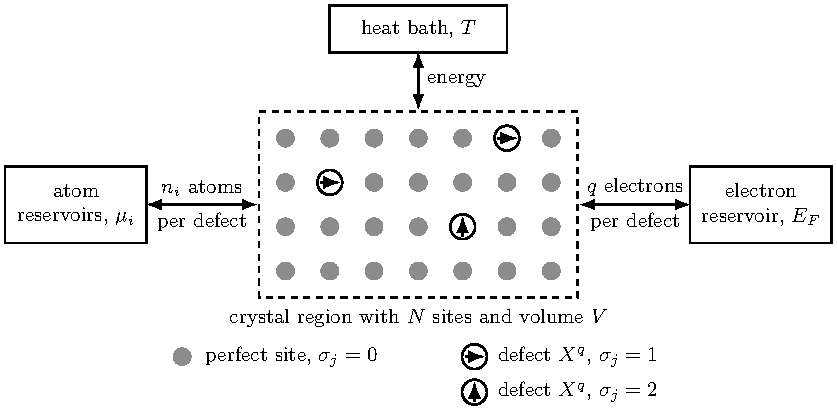
\includegraphics{figures/defect-model}
\caption{Lattice model of a crystal region with $N$ sites in contact with a
heat bath, atom reservoirs and an electron reservoir. Filled circles:
perfect sites. Open circles with an arrow: defects $X^q$, with the arrow
direction as the internal state for $g_X=2$.}
\label{fig:model}
\end{figure}

\paragraph{Defect configuration.}
The model contains one type of defect, the defect $X$ in the
\textcolor{blue}{charge state} $q$, written $X^q$. Each site is either
perfect or holds one defect. A defect at a given site has $g_X$
\textcolor{blue}{internal states} of equal energy, for example the
symmetry-equivalent orientations of a split interstitial or the two spin
directions of an unpaired electron. \textcolor{red}{Here, $\sigma_j$ denotes
the state of site $j$,}
\begin{equation*}
    \sigma_j=
    \begin{cases}
        0, & \text{site $j$ is perfect},\\
        1,\dots,g_X, & \text{site $j$ holds a defect in the internal state
        $\sigma_j$}.
    \end{cases}
\end{equation*}
The \textcolor{blue}{defect configuration}
\begin{equation*}
    \sigma=(\sigma_1,\sigma_2,\dots,\sigma_N)
\end{equation*}
lists the states of all the sites, so the model has $(g_X+1)^N$
configurations. \textcolor{red}{Here, $N_X(\sigma)$ denotes the number of
defects in the configuration $\sigma$,}
\begin{equation*}
    N_X(\sigma)=\sum_{j=1}^{N}\big(1-\delta_{\sigma_j,0}\big),
\end{equation*}
where $\delta_{\sigma_j,0}$ equals one for a perfect site and zero for a
site with a defect.

\paragraph{Exchange with the reservoirs.}
The formation of one defect moves $n_i$ atoms of species $i$ from the
reservoir into the crystal and releases $q$ electrons into the electron
reservoir. A negative $n_i$ removes atoms, as for a vacancy. The crystal
exchanges atoms and electrons with the reservoirs only by forming or
removing defects. \textcolor{red}{Here, $N_i$ and $N_e$ denote the numbers
of atoms of species $i$ and of electrons in the perfect crystal, and
$N_{i,\sigma}$ and $N_{e,\sigma}$ denote the numbers in the configuration
$\sigma$,}
\begin{equation}
    \boxed{N_{i,\sigma}=N_i+n_i\,N_X(\sigma),\qquad
    N_{e,\sigma}=N_e-q\,N_X(\sigma).}
    \label{eq:numbers}
\end{equation}
The particle numbers therefore depend on the configuration only through the
number of defects.

\paragraph{Microstates and the energy of a microstate.}
A configuration fixes where the defects are, but not the motion of the
nuclei or the state of the electrons. With $\sigma$ held fixed, the nuclei
vibrate about the relaxed positions that belong to $\sigma$, and the crystal
has a set of energy eigenstates. \textcolor{red}{Here, $\nu$ labels these
eigenstates, and the pair $(\sigma,\nu)$ labels a microstate in place of the
index $i$ of the note, because $i$ labels the species here.} The energy of
the microstate $(\sigma,\nu)$ has three parts,
\begin{equation}
    \boxed{U_{\sigma\nu}=E^{\text{stat}}_{\sigma}
    +E^{\text{vib}}_{\sigma\nu}+E^{\text{el}}_{\sigma\nu}.}
    \label{eq:energy}
\end{equation}
\begin{itemize}
    \item The \textcolor{blue}{static energy} $E^{\text{stat}}_{\sigma}$ is
    the energy of the crystal with the nuclei at rest at the relaxed
    positions and the electrons in the ground state. This energy is the
    total energy $E_{\text{tot}}$ of a DFT calculation. The static energy
    contains the kinetic energy of the electrons and all the Coulomb
    interactions between the electrons and the nuclei, so the energy of the
    chemical bonds is part of the static energy and not a separate term.
    \item The \textcolor{blue}{vibrational energy}
    $E^{\text{vib}}_{\sigma\nu}$ is the energy of the nuclear motion. In the
    harmonic approximation,
    \begin{equation*}
        E^{\text{vib}}_{\sigma\nu}
        =\sum_k\hbar\omega_{\sigma,k}\Big(\nu_k+\frac12\Big),
    \end{equation*}
    where $\omega_{\sigma,k}$ is the frequency of the phonon mode $k$ of the
    crystal in the configuration $\sigma$, and $\nu_k=0,1,2,\dots$ is the
    occupation number of the mode.
    \item The \textcolor{blue}{electronic excitation energy}
    $E^{\text{el}}_{\sigma\nu}$ is the energy of the electrons above the
    ground state, and vanishes in the electronic ground state.
\end{itemize}
This decomposition is the Born--Oppenheimer picture of a crystal. The
derivation of Section~4 uses only the labels $(\sigma,\nu)$ and the energies
$U_{\sigma\nu}$, so the result does not depend on the harmonic
approximation.

\paragraph{The two assumptions of the model.}
The model rests on two assumptions, and Section~4 gives the mathematical
form of each.
\begin{itemize}
    \item \textbf{Assumption 1, separation into configurations.} Every
    microstate belongs to exactly one configuration $\sigma$. This
    assumption holds when the energy barrier for a defect to hop to another
    site, or to change the internal state, is large compared with $k_BT$.
    The crystal then vibrates many times within one configuration before the
    configuration changes.
    \item \textbf{Assumption 2, non-interacting defects.} The defects are
    far apart, so each defect changes the crystal by the same amount,
    whatever the positions of the other defects.
\end{itemize}
These two statements are assumptions about the crystal and cannot be
derived. All the results of Sections~4 and~5 are exact consequences of the
two assumptions. Sections~6 and~7 add approximations, each with an error
bound.

\section{The Grand Canonical Ensemble of the Model}

\paragraph{Distribution from the entropy maximization.}
The crystal exchanges energy, atoms and electrons with the reservoirs, so
the constrained averages are the energy, the number of atoms of each
species and the number of electrons. The maximum of the Gibbs--Shannon
entropy for these constraints is the grand canonical distribution of
Section~5 of the note. The distribution has one term $\mu_iN_i$ for each
species, as in Section~5.5 of the note, and the term $E_FN_e$ for the
electrons,
\begin{equation}
    \boxed{p_{\sigma\nu}=\frac{1}{\Xi}\,
    e^{-\beta\left(U_{\sigma\nu}-\sum_i\mu_iN_{i,\sigma}-E_FN_{e,\sigma}\right)},
    \qquad
    \Xi=\sum_{\sigma}\sum_{\nu}
    e^{-\beta\left(U_{\sigma\nu}-\sum_i\mu_iN_{i,\sigma}-E_FN_{e,\sigma}\right)},}
    \label{eq:ensemble}
\end{equation}
where $p_{\sigma\nu}$ is the probability of the microstate $(\sigma,\nu)$,
$\Xi$ is the grand canonical partition function and $\beta=1/(k_BT)$.

\paragraph{Grand potential and conjugate variables.}
The thermodynamic potential of the ensemble is the grand potential of
Section~5.2 of the note,
\begin{equation}
    \boxed{\Phi(T,V,\{\mu_i\},E_F)=-k_BT\ln\Xi
    =U-TS-\sum_i\mu_i\langle N_{i,\sigma}\rangle-E_F\langle N_{e,\sigma}\rangle,}
    \label{eq:phi-def}
\end{equation}
where $U$ is the internal energy, $S$ is the entropy, and
$\langle N_{i,\sigma}\rangle$ and $\langle N_{e,\sigma}\rangle$ are the
average numbers of atoms and electrons in the crystal. The differential of
the grand potential is
\begin{equation}
    \boxed{d\Phi=-S\,dT-P\,dV-\sum_i\langle N_{i,\sigma}\rangle\,d\mu_i
    -\langle N_{e,\sigma}\rangle\,dE_F,}
    \label{eq:dphi-general}
\end{equation}
where $P$ is the pressure. Each natural variable therefore has one conjugate
variable, the entropy for $T$, the pressure for $V$, the number of atoms of
species $i$ for $\mu_i$ and the number of electrons for $E_F$. The task is
to evaluate $\Xi$ for the model and to read off the four conjugate
variables.

\section{Evaluation of the Partition Function}

\paragraph{Order of the sums.}
The partition function of Eq.~\eqref{eq:ensemble} is a double sum. The inner
sum runs over the states $\nu$ of one configuration, and the outer sum runs
over the configurations $\sigma$. Figure~\ref{fig:basins} shows this
grouping, with each well as one configuration and each ladder as the states
$\nu$ of that configuration.

\begin{figure}[H]
\centering
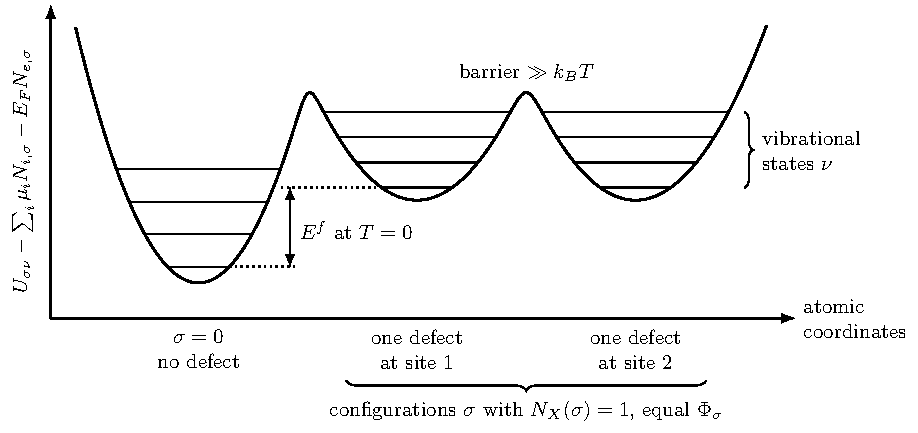
\includegraphics{figures/defect-basins}
\caption{Grouping of the microstates into configurations. Each well: one
defect configuration $\sigma$. Horizontal lines: vibrational states $\nu$ of
the crystal held in that configuration. Offset between the lowest levels:
formation energy at $T=0$.}
\label{fig:basins}
\end{figure}

\paragraph{Step 1: the sum over the states $\nu$ of one configuration.}
The particle numbers do not depend on $\nu$, so the reservoir terms come out
of the inner sum,
\begin{equation*}
    \sum_{\nu}
    e^{-\beta\left(U_{\sigma\nu}-\sum_i\mu_iN_{i,\sigma}-E_FN_{e,\sigma}\right)}
    =e^{\beta\left(\sum_i\mu_iN_{i,\sigma}+E_FN_{e,\sigma}\right)}
    \sum_{\nu}e^{-\beta U_{\sigma\nu}}.
\end{equation*}
The remaining sum adds the Boltzmann factors of all the states of the
crystal held in the configuration $\sigma$, at fixed particle numbers and
fixed volume. This sum is the canonical partition function of Section~3 of
the note. \textcolor{red}{Here, $Z_\sigma$ and $F_\sigma$ denote the
canonical partition function and the Helmholtz free energy of the crystal
held in the configuration $\sigma$,}
\begin{equation*}
    Z_\sigma=\sum_{\nu}e^{-\beta U_{\sigma\nu}},
    \qquad
    F_\sigma=-k_BT\ln Z_\sigma.
\end{equation*}
The free energy $F_\sigma$ contains an entropy, because the sum counts many
states. With the probability of the state $\nu$ within the configuration,
\begin{equation*}
    p_{\nu|\sigma}=\frac{e^{-\beta U_{\sigma\nu}}}{Z_\sigma},
\end{equation*}
the mean energy $U_\sigma$ and the entropy $S_\sigma$ of the crystal held in
the configuration $\sigma$ are
\begin{align*}
    U_\sigma&=\sum_\nu p_{\nu|\sigma}\,U_{\sigma\nu},\\
    S_\sigma&=-k_B\sum_\nu p_{\nu|\sigma}\ln p_{\nu|\sigma}
    =k_B\sum_\nu p_{\nu|\sigma}\big(\beta U_{\sigma\nu}+\ln Z_\sigma\big)
    =\frac{U_\sigma}{T}+k_B\ln Z_\sigma,
\end{align*}
so that
\begin{equation*}
    F_\sigma=-k_BT\ln Z_\sigma=U_\sigma-TS_\sigma.
\end{equation*}
\textcolor{red}{Here, $\Phi_\sigma$ denotes the grand potential of the
crystal held in the configuration $\sigma$,}
\begin{equation*}
    \Phi_\sigma=F_\sigma-\sum_i\mu_iN_{i,\sigma}-E_FN_{e,\sigma}.
\end{equation*}
With these definitions, the partition function becomes
\begin{equation}
    \boxed{\Xi=\sum_{\sigma}e^{-\beta\Phi_\sigma}.}
    \label{eq:xi-sigma}
\end{equation}
Step~1 is exact under Assumption~1, which is the statement that the labels
$(\sigma,\nu)$ cover every microstate exactly once. The grand potentials
$\Phi_{\text{bulk}}$ and $\Phi[X^q]$ of Section~1 of the defect notes are
$\Phi_\sigma$ for the perfect configuration and for a configuration with
one defect.

\paragraph{The free energy of one configuration for harmonic vibrations.}
For harmonic vibrations with the electrons in the ground state, the sum
over $\nu$ runs over every occupation number $\nu_k$ independently, and each
mode contributes a geometric series,
\begin{align*}
    Z_\sigma
    &=e^{-\beta E^{\text{stat}}_\sigma}\prod_k\sum_{\nu_k=0}^{\infty}
    e^{-\beta\hbar\omega_{\sigma,k}\left(\nu_k+\frac12\right)}\\
    &=e^{-\beta E^{\text{stat}}_\sigma}\prod_k
    \frac{e^{-\beta\hbar\omega_{\sigma,k}/2}}{1-e^{-\beta\hbar\omega_{\sigma,k}}}
    =e^{-\beta E^{\text{stat}}_\sigma}\prod_k
    \frac{1}{2\sinh\!\big(\beta\hbar\omega_{\sigma,k}/2\big)}.
\end{align*}
The free energy is therefore
\begin{equation}
    \boxed{F_\sigma=E^{\text{stat}}_\sigma
    +k_BT\sum_k\ln\!\Big[2\sinh\!\Big(\frac{\hbar\omega_{\sigma,k}}{2k_BT}\Big)\Big].}
    \label{eq:harmonic}
\end{equation}
For $T\to0$, each logarithm tends to $\hbar\omega_{\sigma,k}/(2k_BT)$, and
\begin{equation*}
    F_\sigma\to E^{\text{stat}}_\sigma+\sum_k\frac{\hbar\omega_{\sigma,k}}{2},
\end{equation*}
which is the static energy plus the zero-point energy, the result
$F=U=E_{\text{tot}}+E_{\text{ZPE}}$ of Section~1 of the defect notes.

\paragraph{Step 2: non-interacting defects and the formation energy.}
\textcolor{red}{Here, $F_{\text{bulk}}$ denotes $F_\sigma$ of the perfect
configuration, $F[X^q]$ denotes $F_\sigma$ of a configuration with one
defect, and $\Delta F$ denotes the difference,}
\begin{equation*}
    \Delta F=F[X^q]-F_{\text{bulk}}.
\end{equation*}
All the sites of the lattice are equivalent, and the internal states have
equal energies, so $\Delta F$ does not depend on the site or on the internal
state of the defect. Assumption~2 states that every further defect changes
the free energy by the same amount,
\begin{equation}
    \boxed{F_\sigma=F_{\text{bulk}}+N_X(\sigma)\,\Delta F.}
    \label{eq:assumption2}
\end{equation}
This assumption requires that the static energies of distant defects add,
and that each defect changes the phonon frequencies only in the surroundings
of the defect. The assumption fails at high concentrations and for charged
defects with an unscreened Coulomb interaction. The particle numbers of
Eq.~\eqref{eq:numbers} then give
\begin{align*}
    \Phi_\sigma
    &=F_{\text{bulk}}+N_X(\sigma)\,\Delta F
    -\sum_i\mu_i\big[N_i+n_i\,N_X(\sigma)\big]
    -E_F\big[N_e-q\,N_X(\sigma)\big]\\
    &=\Big[F_{\text{bulk}}-\sum_i\mu_iN_i-E_FN_e\Big]
    +N_X(\sigma)\Big[\Delta F-\sum_i\mu_in_i+qE_F\Big].
\end{align*}
The first bracket is the grand potential $\Phi_{\text{bulk}}$ of the perfect
configuration. The second bracket is the \textcolor{blue}{formation energy}
of one defect,
\begin{equation}
    \boxed{E^f[X^q]=F[X^q]-F_{\text{bulk}}-\sum_i\mu_in_i+qE_F
    =\Phi[X^q]-\Phi_{\text{bulk}},}
    \label{eq:Ef}
\end{equation}
the definition of Section~1 of the defect notes. The formation energy is a
function of the natural variables. The temperature and the volume enter
through $\Delta F$, and the chemical potentials and the Fermi level enter
through the reservoir terms. \textcolor{red}{For brevity, $E^f$ replaces
$E^f[X^q]$ until Section~9, because only one type of defect appears.} Every
configuration therefore has
\begin{equation}
    \boxed{\Phi_\sigma=\Phi_{\text{bulk}}+N_X(\sigma)\,E^f.}
    \label{eq:phi-sigma}
\end{equation}

\paragraph{Step 3: the sum over the configurations.}
Equations~\eqref{eq:xi-sigma} and~\eqref{eq:phi-sigma} give
\begin{equation*}
    \Xi=e^{-\beta\Phi_{\text{bulk}}}\sum_{\sigma}e^{-\beta E^f N_X(\sigma)}.
\end{equation*}
The number of defects is a sum over the sites, so the exponential is a
product over the sites. The sum over $\sigma$ is a sum over every $\sigma_j$
independently, and the sum of the products is the product of the sums,
\begin{align*}
    \sum_{\sigma}e^{-\beta E^f N_X(\sigma)}
    &=\sum_{\sigma_1=0}^{g_X}\cdots\sum_{\sigma_N=0}^{g_X}\;
    \prod_{j=1}^{N}e^{-\beta E^f\left(1-\delta_{\sigma_j,0}\right)}\\
    &=\prod_{j=1}^{N}\;\sum_{\sigma_j=0}^{g_X}
    e^{-\beta E^f\left(1-\delta_{\sigma_j,0}\right)}\\
    &=\prod_{j=1}^{N}\Big(1+g_X\,e^{-\beta E^f}\Big)
    =\Big(1+g_X\,e^{-\beta E^f}\Big)^{N}.
\end{align*}
Each site contributes the weight $1$ for the perfect state and the weight
$e^{-\beta E^f}$ for each of the $g_X$ defect states. \textcolor{red}{Here,
$\zeta_X$ denotes the total weight of the defect states of one site,}
\begin{equation*}
    \zeta_X=g_X\,e^{-E^f/k_BT}.
\end{equation*}
The partition function and the grand potential of the model are
\begin{equation}
    \boxed{\Xi=e^{-\Phi_{\text{bulk}}/k_BT}\,\big(1+\zeta_X\big)^{N},
    \qquad
    \Phi=\Phi_{\text{bulk}}-Nk_BT\ln\big(1+\zeta_X\big).}
    \label{eq:result}
\end{equation}
The result uses no Stirling approximation and no dilute limit. The crystal
behaves as $N$ independent sites, each with one perfect state and $g_X$
defect states.

\section{Conjugate Variables}

\paragraph{State of one site and the defect concentration.}
The probability of a configuration is the sum of $p_{\sigma\nu}$ over $\nu$,
\begin{equation*}
    p_\sigma=\sum_\nu p_{\sigma\nu}=\frac{e^{-\beta\Phi_\sigma}}{\Xi}
    =\prod_{j=1}^{N}
    \frac{e^{-\beta E^f\left(1-\delta_{\sigma_j,0}\right)}}{1+\zeta_X}.
\end{equation*}
The probability is a product over the sites, so the sites are statistically
independent. A site is perfect with the probability $1/(1+\zeta_X)$ and
holds a defect in a given internal state with the probability
$e^{-\beta E^f}/(1+\zeta_X)$. The \textcolor{blue}{defect concentration} is
the average number of defects per site,
\begin{equation}
    \boxed{c\equiv\frac{\langle N_X\rangle}{N}=\frac{\zeta_X}{1+\zeta_X}
    =\frac{1}{1+g_X^{-1}\,e^{E^f/k_BT}}.}
    \label{eq:c}
\end{equation}
The concentration has the form of the Fermi--Dirac occupation, because a
site holds at most one defect, and never exceeds one
(Fig.~\ref{fig:concentration}b). The same concentration follows from a
derivative of the grand potential,
\begin{equation*}
    \frac{\partial\Phi}{\partial E^f}\bigg|_{T}
    =-Nk_BT\,\frac{1}{1+\zeta_X}\,\frac{\partial\zeta_X}{\partial E^f}
    =N\,\frac{\zeta_X}{1+\zeta_X}=Nc,
\end{equation*}
so the formation energy and the number of defects are a conjugate pair.

\begin{figure}[H]
\centering
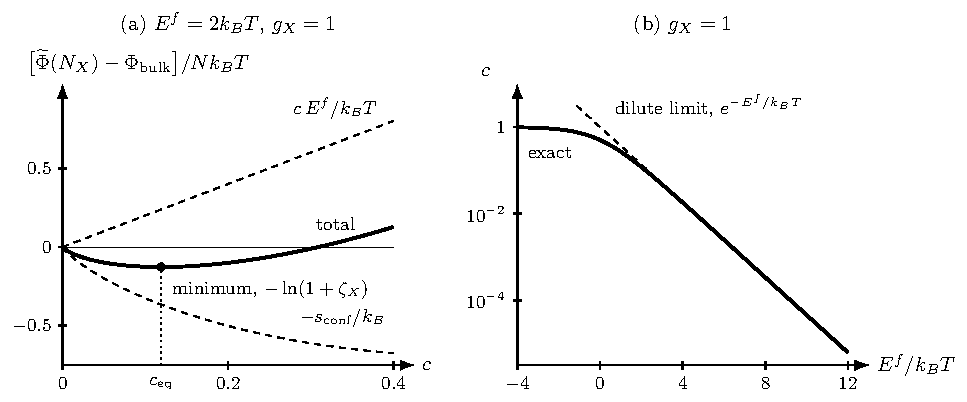
\includegraphics{figures/defect-concentration}
\caption{(a) Constrained grand potential per site of Section~7 against the
defect concentration for $E^f=2k_BT$ and $g_X=1$, with the energy term, the
entropy term and the total. Dot: minimum at the equilibrium concentration.
(b) Defect concentration against $E^f/k_BT$ for $g_X=1$. Solid line: exact
result. Dashed line: dilute limit.}
\label{fig:concentration}
\end{figure}

\paragraph{Differential of the grand potential.}
\textcolor{red}{Here, $\Phi_{\text{def}}$ denotes the defect part of the
grand potential,}
\begin{equation*}
    \Phi_{\text{def}}=\Phi-\Phi_{\text{bulk}}=-Nk_BT\ln\big(1+\zeta_X\big).
\end{equation*}
The defect part depends on the natural variables through $E^f$ and through
the explicit temperature, so
\begin{equation*}
    d\Phi=d\Phi_{\text{bulk}}
    +\frac{\partial\Phi_{\text{def}}}{\partial T}\bigg|_{E^f}dT+Nc\,dE^f.
\end{equation*}
The explicit temperature derivative is
\begin{align*}
    \frac{\partial\Phi_{\text{def}}}{\partial T}\bigg|_{E^f}
    &=-Nk_B\ln\big(1+\zeta_X\big)
    -Nk_BT\,\frac{1}{1+\zeta_X}\,\frac{\zeta_X E^f}{k_BT^2}\\
    &=-Nk_B\ln\big(1+\zeta_X\big)-Nc\,\frac{E^f}{T}.
\end{align*}
Equation~\eqref{eq:c} gives the two relations
\begin{equation}
    \boxed{\ln\big(1+\zeta_X\big)=-\ln(1-c),
    \qquad
    \frac{E^f}{k_BT}=\ln g_X-\ln c+\ln(1-c),}
    \label{eq:identities}
\end{equation}
and the derivative becomes
\begin{align*}
    \frac{\partial\Phi_{\text{def}}}{\partial T}\bigg|_{E^f}
    &=-Nk_B\big[-\ln(1-c)+c\ln g_X-c\ln c+c\ln(1-c)\big]\\
    &=-Nk_B\big[c\ln g_X-c\ln c-(1-c)\ln(1-c)\big]
    =-N\,s_{\text{conf}}(c),
\end{align*}
with the \textcolor{blue}{configurational entropy} per site
\begin{equation}
    \boxed{s_{\text{conf}}(c)=k_B\big[c\ln g_X-c\ln c-(1-c)\ln(1-c)\big].}
    \label{eq:sconf}
\end{equation}
The formation energy of Eq.~\eqref{eq:Ef} has the differential
\begin{equation*}
    dE^f=-S^f\,dT-\frac{B_TV^f}{V}\,dV-\sum_in_i\,d\mu_i+q\,dE_F,
\end{equation*}
which defines the \textcolor{blue}{formation entropy} $S^f$ and the
\textcolor{blue}{formation volume} $V^f$ of one defect,
\begin{equation*}
    S^f=-\frac{\partial E^f}{\partial T}\bigg|_{V}
    =-\frac{\partial\Delta F}{\partial T}\bigg|_{V},
    \qquad
    V^f=-\frac{V}{B_T}\,\frac{\partial E^f}{\partial V}\bigg|_{T},
    \qquad
    B_T=-V\,\frac{\partial P_{\text{bulk}}}{\partial V}\bigg|_{T},
\end{equation*}
where $B_T$ is the isothermal bulk modulus of the perfect crystal. The
formation entropy is the change of the vibrational and electronic entropy
$S_\sigma$ when one defect forms. The perfect configuration has fixed
particle numbers, so
\begin{equation*}
    d\Phi_{\text{bulk}}=-S_{\text{bulk}}\,dT-P_{\text{bulk}}\,dV
    -\sum_iN_i\,d\mu_i-N_e\,dE_F,
\end{equation*}
where $S_{\text{bulk}}$ and $P_{\text{bulk}}$ are the entropy and the
pressure of the perfect crystal. The sum of the three contributions is
\begin{equation}
    \boxed{
    \begin{aligned}
    d\Phi={}&-\big[S_{\text{bulk}}+N\,s_{\text{conf}}(c)+Nc\,S^f\big]\,dT
    -\Big[P_{\text{bulk}}+Nc\,\frac{B_TV^f}{V}\Big]\,dV\\
    &-\sum_i\big[N_i+n_i\,Nc\big]\,d\mu_i
    -\big[N_e-q\,Nc\big]\,dE_F.
    \end{aligned}}
    \label{eq:dphi}
\end{equation}
The comparison with Eq.~\eqref{eq:dphi-general} gives all the conjugate
variables, which Table~\ref{tab:conjugates} lists.

\begin{table}[H]
\centering
\caption{Conjugate variables of the grand potential of the lattice model.}
\label{tab:conjugates}
\renewcommand{\arraystretch}{1.9}
\begin{tabular}{|c|c|c|c|}
\hline
Natural variable & Conjugate variable & Perfect crystal & Defects \\ \hline
$T$ & $S=-\dfrac{\partial\Phi}{\partial T}$ & $S_{\text{bulk}}$
    & $N\,s_{\text{conf}}(c)+Nc\,S^f$ \\ \hline
$V$ & $P=-\dfrac{\partial\Phi}{\partial V}$ & $P_{\text{bulk}}$
    & $Nc\,\dfrac{B_TV^f}{V}$ \\ \hline
$\mu_i$ & $\langle N_{i,\sigma}\rangle=-\dfrac{\partial\Phi}{\partial\mu_i}$
    & $N_i$ & $n_i\,Nc$ \\ \hline
$E_F$ & $\langle N_{e,\sigma}\rangle=-\dfrac{\partial\Phi}{\partial E_F}$
    & $N_e$ & $-q\,Nc$ \\ \hline
\end{tabular}
\end{table}

\paragraph{Particle numbers.}
The crystal holds the atoms and electrons of the perfect crystal, plus
$n_i$ atoms and minus $q$ electrons for each of the $Nc$ defects. The
derivatives of $\Phi$ therefore agree with the direct averages of
Eq.~\eqref{eq:numbers},
\begin{equation}
    \boxed{\langle N_{i,\sigma}\rangle=N_i+n_i\,Nc,
    \qquad
    \langle N_{e,\sigma}\rangle=N_e-q\,Nc.}
\end{equation}

\paragraph{Entropy and the origin of the configurational entropy.}
The entropy has three contributions,
\begin{equation}
    \boxed{S=S_{\text{bulk}}+Nc\,S^f+N\,s_{\text{conf}}(c).}
    \label{eq:S}
\end{equation}
The first two contributions are vibrational and electronic. The third
contribution is the entropy of the distribution over the configurations.
The probability of a microstate is the product
$p_{\sigma\nu}=p_\sigma\,p_{\nu|\sigma}$, so the Gibbs--Shannon entropy
splits into two parts,
\begin{align*}
    S&=-k_B\sum_{\sigma}\sum_{\nu}p_\sigma\,p_{\nu|\sigma}
    \big[\ln p_\sigma+\ln p_{\nu|\sigma}\big]\\
    &=-k_B\sum_{\sigma}p_\sigma\ln p_\sigma
    +\sum_{\sigma}p_\sigma\Big[-k_B\sum_\nu p_{\nu|\sigma}\ln p_{\nu|\sigma}\Big]\\
    &=-k_B\sum_{\sigma}p_\sigma\ln p_\sigma+\sum_{\sigma}p_\sigma\,S_\sigma.
\end{align*}
The second part is the average of the entropy $S_\sigma$ of Step~1. With
Eq.~\eqref{eq:assumption2}, $S_\sigma=S_{\text{bulk}}+N_X(\sigma)\,S^f$, and
the average is $S_{\text{bulk}}+Nc\,S^f$. The first part is the entropy of
the configurations. The sites are independent, so this entropy is $N$ times
the entropy of one site (Section~3.2 of the note). One site is perfect with
the probability $1-c$ and is in each of the $g_X$ defect states with the
probability $c/g_X$, so
\begin{align*}
    -k_B\sum_{\sigma}p_\sigma\ln p_\sigma
    &=-Nk_B\Big[(1-c)\ln(1-c)+g_X\,\frac{c}{g_X}\ln\frac{c}{g_X}\Big]\\
    &=Nk_B\big[c\ln g_X-c\ln c-(1-c)\ln(1-c)\big]
    =N\,s_{\text{conf}}(c).
\end{align*}
The direct evaluation therefore reproduces Eq.~\eqref{eq:S}. The
configurational entropy is not an additional postulate. This entropy is the
part of the Gibbs--Shannon entropy that belongs to the distribution over the
configurations, and the vibrational entropy is the part that belongs to the
states within one configuration.

\paragraph{Internal energy.}
The internal energy follows from Eq.~\eqref{eq:phi-def},
\begin{equation*}
    U=\Phi+TS+\sum_i\mu_i\langle N_{i,\sigma}\rangle
    +E_F\langle N_{e,\sigma}\rangle.
\end{equation*}
The terms of the perfect crystal add up to the internal energy
$U_{\text{bulk}}$ of the perfect crystal. For the defect terms,
Eq.~\eqref{eq:identities} gives
\begin{equation*}
    -k_BT\ln\big(1+\zeta_X\big)+T\,s_{\text{conf}}(c)
    =k_BT\,c\,\big[\ln g_X-\ln c+\ln(1-c)\big]=c\,E^f,
\end{equation*}
so that
\begin{align*}
    U&=U_{\text{bulk}}+Nc\Big[E^f+TS^f+\sum_i\mu_in_i-qE_F\Big]\\
    &=U_{\text{bulk}}+Nc\,\big[\Delta F+TS^f\big].
\end{align*}
\textcolor{red}{Here, $\Delta U=\Delta F+TS^f$ denotes the change of the
internal energy when one defect forms, which contains the static, the
vibrational and the electronic energy.} The internal energy is
\begin{equation}
    \boxed{U=U_{\text{bulk}}+Nc\,\Delta U.}
\end{equation}
The internal energy contains no reservoir term and no configurational term,
because the arrangement of the defects on the sites costs no energy.

\paragraph{Pressure and the meaning of the formation volume.}
The pressure of the crystal is
\begin{equation}
    \boxed{P=P_{\text{bulk}}+Nc\,\frac{B_TV^f}{V}.}
\end{equation}
At fixed volume, each defect raises the pressure by $B_TV^f/V$. If the
crystal is released to the original pressure $P_{\text{bulk}}$, the volume
changes by $\Delta V$, with
\begin{equation*}
    -\frac{B_T}{V}\,\Delta V+Nc\,\frac{B_TV^f}{V}=0
    \qquad\Longrightarrow\qquad
    \Delta V=Nc\,V^f
\end{equation*}
to first order in $c$. The formation volume $V^f$ is therefore the volume
change per defect at fixed pressure, with the exchanged atoms in the
reservoirs. For a vacancy, $V^f$ does not include the volume of the removed
atom, because this atom is in the reservoir.

\paragraph{Fluctuation of the number of defects.}
The number of defects is a sum of $N$ independent site variables, each equal
to one with the probability $c$ and to zero with the probability $1-c$. The
variance of one site variable is $c(1-c)$, and the variances of independent
variables add, so
\begin{equation}
    \boxed{\mathrm{Var}(N_X)=Nc\,(1-c),
    \qquad
    \frac{\sqrt{\mathrm{Var}(N_X)}}{\langle N_X\rangle}
    =\sqrt{\frac{1-c}{Nc}}.}
    \label{eq:var}
\end{equation}
The same variance follows from the fluctuation formula of Section~5.1 of the
note, with $-E^f$ in the role of the chemical potential,
\begin{equation*}
    \mathrm{Var}(N_X)=-k_BT\,\frac{\partial\langle N_X\rangle}{\partial E^f}\bigg|_{T}
    =-k_BT\,N\,\frac{\partial c}{\partial E^f}\bigg|_{T}=Nc\,(1-c).
\end{equation*}
For $N=10^{22}$ sites and $c=10^{-6}$, the relative fluctuation is
$10^{-8}$, so the number of defects is sharply defined.

\section{Approximations with Error Bounds}

\paragraph{The dilute limit.}
For $\zeta_X\geq0$, the product $(1-\zeta_X)(1+\zeta_X)=1-\zeta_X^2$ does
not exceed one, so
\begin{equation*}
    1-\zeta_X\;\leq\;\frac{1}{1+\zeta_X}\;\leq\;1.
\end{equation*}
Multiplication by $\zeta_X$ bounds the concentration of Eq.~\eqref{eq:c},
and integration of the three terms from $0$ to $\zeta_X$ bounds the
logarithm of Eq.~\eqref{eq:result},
\begin{equation}
    \boxed{\zeta_X-\zeta_X^2\;\leq\;c\;\leq\;\zeta_X,
    \qquad
    \zeta_X-\frac{\zeta_X^2}{2}\;\leq\;\ln\big(1+\zeta_X\big)\;\leq\;\zeta_X.}
\end{equation}
The \textcolor{blue}{dilute limit} keeps the first order in $\zeta_X$,
\begin{equation}
    \boxed{c\approx g_X\,e^{-E^f/k_BT},
    \qquad
    \Phi\approx\Phi_{\text{bulk}}-Nk_BT\,c,}
    \label{eq:dilute}
\end{equation}
with a relative error of at most $\zeta_X$ in each expression. These
results are Eqs.~(41) and~(40) of Freysoldt \textit{et
al.}~\cite{freysoldt}. For $E^f=1$~eV, $T=1000$~K and $g_X=1$, the exponent
is $E^f/k_BT=11.6$ and $\zeta_X=9\times10^{-6}$, so the dilute limit is
accurate to one part in $10^5$. The configurational entropy has the dilute
form
\begin{equation}
    \boxed{s_{\text{conf}}(c)\approx k_B\big[c\ln g_X-c\ln c+c\big],}
    \label{eq:sconf-dilute}
\end{equation}
which is Eq.~(7) of the review. The error is the function
\begin{equation*}
    h(c)=c+(1-c)\ln(1-c),
    \qquad
    h'(c)=-\ln(1-c)\geq0,
    \qquad
    h''(c)=\frac{1}{1-c}\leq2\quad\text{for }c\leq\tfrac12,
\end{equation*}
with $h(0)=h'(0)=0$, so that $0\leq h(c)\leq c^2$ for $c\leq1/2$. The dilute
form therefore overestimates $s_{\text{conf}}$ by at most $k_Bc^2$.

\paragraph{The formation energy at $T=0$ in the concentration.}
A DFT calculation gives the formation energy at $T=0$. At fixed volume,
chemical potentials and Fermi level, the definition of the formation
entropy gives the exact relation
\begin{equation*}
    E^f(T)=E^f(0)-\int_0^{T}S^f(T')\,dT'.
\end{equation*}
\textcolor{red}{Here, $\bar S^f$ denotes the formation entropy averaged over
the temperature,}
\begin{equation*}
    \bar S^f(T)=\frac{1}{T}\int_0^{T}S^f(T')\,dT'.
\end{equation*}
The dilute concentration of Eq.~\eqref{eq:dilute} becomes
\begin{equation}
    \boxed{c\approx g_X\,e^{\bar S^f(T)/k_B}\,e^{-E^f(0)/k_BT}.}
    \label{eq:c-zeroK}
\end{equation}
The formation energy at $T=0$ gives the last factor. The factor
$e^{\bar S^f/k_B}$ is the exact price of the neglected temperature
dependence. Formation entropies of a few $k_B$ are typical, and the value
$2.4\,k_B$ quoted in the review for the vacancy in aluminum corresponds to a
factor of $e^{2.4}=11$. If a reservoir is a phase with a chemical potential
that depends on the temperature, $E^f$ changes along the path by
\begin{equation*}
    \frac{dE^f}{dT}=-S^f-\sum_in_i\,\frac{d\mu_i}{dT},
\end{equation*}
and Eq.~\eqref{eq:c-zeroK} holds with $-dE^f/dT$ in place of $S^f$.

\section{The Minimization Route of the Review}

\paragraph{The constrained grand potential.}
Freysoldt \textit{et al.}~\cite{freysoldt} obtained the concentration from
the minimum of a potential at a fixed number of defects. This potential
follows from the sum of Eq.~\eqref{eq:xi-sigma}, with the configurations
grouped by the number of defects,
\begin{equation*}
    \Xi=\sum_{N_X=0}^{N}\;\sum_{\sigma:\,N_X(\sigma)=N_X}e^{-\beta\Phi_\sigma}
    =\sum_{N_X=0}^{N}W(N_X)\,e^{-\beta\left(\Phi_{\text{bulk}}+N_XE^f\right)},
\end{equation*}
where $W(N_X)$ is the number of configurations with $N_X$ defects. A
configuration with $N_X$ defects is fixed by the choice of $N_X$ sites out
of $N$ and of one internal state for each defect, so
\begin{equation}
    \boxed{W(N_X)=g_X^{N_X}\,\frac{N!}{N_X!\,(N-N_X)!}.}
\end{equation}
All these configurations have the same $\Phi_\sigma$ and are equally
probable. The entropy of $W$ equally probable configurations is the
microcanonical entropy of Section~2 of the note,
\begin{equation*}
    S_{\text{conf}}(N_X)=k_B\ln W(N_X).
\end{equation*}
\textcolor{red}{Here, $\widetilde{\Phi}(N_X)$ denotes the
\textcolor{blue}{constrained grand potential}, the grand potential of the
ensemble restricted to $N_X$ defects,}
\begin{equation}
    \boxed{\widetilde{\Phi}(N_X)
    =-k_BT\ln\Big[W(N_X)\,e^{-\beta\left(\Phi_{\text{bulk}}+N_XE^f\right)}\Big]
    =\Phi_{\text{bulk}}+N_X\,E^f-T\,S_{\text{conf}}(N_X).}
    \label{eq:constrained}
\end{equation}
The potential $F^{\text{conf}}$ of Eq.~(8) of the review is
$\widetilde{\Phi}(N_X)-\Phi_{\text{bulk}}$ per site. The term $N_XE^f$
contains the reservoir terms, so this potential is a constrained grand
potential and not a Helmholtz free energy.

\paragraph{The largest term of the sum.}
The partition function is a sum of $N+1$ positive terms,
\begin{equation*}
    \Xi=\sum_{N_X=0}^{N}e^{-\beta\widetilde{\Phi}(N_X)}.
\end{equation*}
A sum of $N+1$ positive terms is at least the largest term and at most
$N+1$ times the largest term. The largest term belongs to the smallest
$\widetilde{\Phi}(N_X)$, so the logarithm of the two bounds gives
\begin{equation}
    \boxed{\min_{N_X}\widetilde{\Phi}(N_X)-k_BT\ln(N+1)
    \;\leq\;\Phi\;\leq\;\min_{N_X}\widetilde{\Phi}(N_X).}
    \label{eq:largest}
\end{equation}
The grand potential per site equals the minimum of the constrained
potential per site up to $k_BT\ln(N+1)/N$, which is $5\times10^{-21}\,k_BT$
for $N=10^{22}$. The minimization of the review is therefore exact in the
thermodynamic limit. The sharp distribution of Eq.~\eqref{eq:var} expresses
the same fact.

\paragraph{The Stirling approximation with a bound.}
The logarithm of a factorial is a sum of logarithms. The logarithm is an
increasing function, so each term lies between two integrals,
\begin{equation*}
    \int_{k-1}^{k}\ln t\,dt\;\leq\;\ln k\;\leq\;\int_{k}^{k+1}\ln t\,dt.
\end{equation*}
The sum of the lower bounds from $k=1$ to $n$, and the sum of the upper
bounds from $k=1$ to $n-1$ plus the last term $\ln n$, give
\begin{equation*}
    \int_0^{n}\ln t\,dt\;\leq\;\ln n!\;\leq\;\int_1^{n}\ln t\,dt+\ln n.
\end{equation*}
With the integral $\int\ln t\,dt=t\ln t-t$, the bounds are
\begin{equation}
    \boxed{n\ln n-n\;\leq\;\ln n!\;\leq\;n\ln n-n+1+\ln n.}
    \label{eq:stirling}
\end{equation}
The Stirling formula $\ln n!\approx n\ln n-n$ therefore has an error between
$0$ and $1+\ln n$. For $0<N_X<N$ and $c=N_X/N$, the leading terms of the
three factorials in $W(N_X)$ are
\begin{align*}
    \ln W(N_X)
    &\approx N_X\ln g_X+N\ln N-N_X\ln N_X-(N-N_X)\ln(N-N_X)\\
    &=N\big[c\ln g_X-c\ln c-(1-c)\ln(1-c)\big],
\end{align*}
with a total error of at most $2(1+\ln N)$. The terms $-N$, $+N_X$ and
$+(N-N_X)$ cancel. The constrained potential per site is therefore
\begin{equation}
    \boxed{\frac{\widetilde{\Phi}(N_X)-\Phi_{\text{bulk}}}{N}
    =c\,E^f-T\,s_{\text{conf}}(c)
    +\mathcal{O}\!\Big(\frac{k_BT\ln N}{N}\Big),}
    \label{eq:phi-c}
\end{equation}
with the same $s_{\text{conf}}(c)$ as in Eq.~\eqref{eq:sconf}.

\paragraph{The minimum reproduces the exact result.}
The derivative of the leading term of Eq.~\eqref{eq:phi-c} is
\begin{equation*}
    \frac{d}{dc}\big[c\,E^f-T\,s_{\text{conf}}(c)\big]
    =E^f-k_BT\big[\ln g_X-\ln c+\ln(1-c)\big],
\end{equation*}
and the second derivative, $k_BT\,[1/c+1/(1-c)]$, is positive, so the
stationary point is a minimum (Fig.~\ref{fig:concentration}a). The
derivative vanishes for
\begin{equation*}
    \frac{c}{1-c}=g_X\,e^{-E^f/k_BT}=\zeta_X
    \qquad\Longrightarrow\qquad
    c=\frac{\zeta_X}{1+\zeta_X},
\end{equation*}
which is the concentration of Eq.~\eqref{eq:c}. By
Eq.~\eqref{eq:identities}, the value at the minimum is
\begin{equation*}
    c\,E^f-T\,s_{\text{conf}}(c)=-k_BT\ln\big(1+\zeta_X\big),
\end{equation*}
which is the defect part of Eq.~\eqref{eq:result} per site. The
minimization route therefore agrees with the direct sum. The review used
the dilute entropy of Eq.~\eqref{eq:sconf-dilute} in the minimization, which
gives the dilute results of Eq.~\eqref{eq:dilute}.

\section{Fixed Pressure}

\paragraph{The potential at fixed pressure.}
Experiments fix the pressure and not the volume. The reservoirs fix the
chemical potentials and the Fermi level in both cases. The potential with
the natural variables $(T,P,\{\mu_i\},E_F)$ is the Legendre transform of
$\Phi$ in the volume (Section~4.4 of the note). \textcolor{red}{Here,
$\Phi_P$ denotes this potential,}
\begin{equation*}
    \Phi_P(T,P,\{\mu_i\},E_F)=\Phi+PV,
    \qquad
    P=-\frac{\partial\Phi}{\partial V}\bigg|_{T,\{\mu_i\},E_F}.
\end{equation*}
For a fluid, this potential vanishes identically, because no extensive
variable would fix the size of the system (Section~5.7 of the note). In the
lattice model, the fixed number of sites $N$ fixes the size, so $\Phi_P$ is
a proper potential. The Gibbs energy $G$ of the review is this potential,
because the review subtracted the reservoir terms.

\paragraph{The formation energy at fixed pressure.}
The perfect crystal at the pressure $P$ has the volume $V$, with
\begin{equation*}
    \frac{\partial\Phi_{\text{bulk}}}{\partial V}\bigg|_{V}=-P.
\end{equation*}
A crystal with one defect has the grand potential
$\Phi_{\text{bulk}}(V')+E^f(V')$ at the volume $V'$ and relaxes to the
volume that minimizes the potential at fixed pressure.
\textcolor{red}{Here, $E^f_P$ denotes the formation energy at fixed
pressure,}
\begin{equation*}
    E^f_P=\min_{V'}\Big[\Phi_{\text{bulk}}(V')+E^f(V')+PV'\Big]
    -\Big[\Phi_{\text{bulk}}(V)+PV\Big].
\end{equation*}
With Eq.~\eqref{eq:Ef} written out, this definition reads
\begin{equation*}
    E^f_P=F[X^q](V')-F_{\text{bulk}}(V)+P\,(V'-V)-\sum_i\mu_in_i+qE_F,
\end{equation*}
which is the Gibbs energy of formation $G^f$ of Eq.~(23) of the review. The
expansion of the two terms about the volume $V$ to second order in $V'-V$
uses the definitions of $B_T$ and $V^f$ of Section~5,
\begin{align*}
    \Phi_{\text{bulk}}(V')+PV'
    &\approx\Phi_{\text{bulk}}(V)+PV+\frac{B_T}{2V}\,(V'-V)^2,\\
    E^f(V')&\approx E^f(V)-\frac{B_TV^f}{V}\,(V'-V).
\end{align*}
The sum is a minimum for $V'-V=V^f$, and the value at the minimum gives
\begin{equation}
    \boxed{E^f_P=E^f(V)-\frac{B_T\,(V^f)^2}{2V}.}
    \label{eq:EfP}
\end{equation}
The difference between the two formation energies is proportional to $1/V$
and vanishes for one defect in a large crystal. For $B_T=100$~GPa,
$V^f=10^{-29}$~m$^3$ and a volume of $2\times10^{-29}$~m$^3$ per site, the
difference is $1.6$~eV divided by the number of sites, which is $16$~meV for
a supercell of 100 sites and negligible for a macroscopic crystal. The term
$P\,(V'-V)$ does not appear in Eq.~\eqref{eq:EfP}, because the change of
$F[X^q]$ between the volumes $V$ and $V'$ cancels this term to first order.

\paragraph{Finite concentration at fixed pressure.}
For $N_X$ defects, the same expansion gives the relaxation $V'-V=N_XV^f$ and
a correction of $c\,B_T(V^f)^2/(2v)$ per defect, where $v=V/N$ is the volume
per site. This correction is an interaction between the defects through the
strain of the lattice. The correction is of first order in $c$ and is
neglected under Assumption~2. All the results of Sections~4 to~7 therefore
hold at fixed pressure, with $E^f$ evaluated at the volume of the perfect
crystal at the pressure $P$ and the temperature $T$.

\section{Charge States and the Fermi Level}

\paragraph{Several charge states on the same sites.}
A defect $X$ can take several charge states $q$. \textcolor{red}{From here
on, $E^f[X^q]$ replaces $E^f$, and $g_q$ and $\zeta_q$ replace $g_X$ and
$\zeta_X$ for the charge state $q$.} Each site is then perfect or holds the
defect in one charge state $q$ and one of the $g_q$ internal states. The
derivation of Section~4 goes through unchanged, and each site contributes
the factor $1+\sum_q\zeta_q$, with
\begin{equation*}
    \zeta_q=g_q\,e^{-E^f[X^q]/k_BT}.
\end{equation*}
The grand potential and the concentration $c_q$ of the charge state $q$ are
\begin{equation}
    \boxed{\Phi=\Phi_{\text{bulk}}-Nk_BT\ln\Big(1+\sum_q\zeta_q\Big),
    \qquad
    c_q=\frac{\zeta_q}{1+\sum_{q'}\zeta_{q'}}.}
\end{equation}
The ratio of the concentrations of two charge states is
\begin{equation}
    \boxed{\frac{c_q}{c_{q'}}
    =\frac{g_q}{g_{q'}}\,e^{-\left(E^f[X^q]-E^f[X^{q'}]\right)/k_BT}
    =\frac{g_q}{g_{q'}}\,
    e^{-(q-q')\left[E_F-\varepsilon(q/q')\right]/k_BT},}
\end{equation}
where $\varepsilon(q/q')$ is the charge-state transition level of Section~2
of the defect notes, evaluated with the formation energies at the
temperature $T$. For equal numbers of internal states, the two charge
states have equal concentrations when the Fermi level is at the transition
level. The change of the dominant charge state at the transition level is
spread over a few $k_BT$ in the Fermi level.

\paragraph{The condition that fixes the Fermi level.}
The Fermi level is a natural variable of $\Phi$, set by the electron
reservoir. A real crystal has no external electron reservoir. The electrons
released by the defects enter the bands or other defects, and the crystal
stays neutral. \textcolor{red}{Here, $\mathcal{N}_e$ and $\mathcal{N}_h$
denote the numbers of free electrons and free holes in the bands of the
crystal region.} The neutrality condition is
\begin{equation}
    \boxed{\sum_q q\,N c_q+\mathcal{N}_h-\mathcal{N}_e=0,}
\end{equation}
which is Eq.~(36) of the review. The concentrations $c_q$ and the carrier
numbers depend on $E_F$, so this condition determines $E_F$. The free
carriers add a factor to $\Xi$ that does not depend on the defect
configuration, as long as the carriers and the defects do not interact, so
the defect factor of Eq.~\eqref{eq:result} is unchanged.

\section{Dictionary for the Review}

\paragraph{Translation of the symbols and equations.}
Table~\ref{tab:dictionary} relates the symbols and equations of Freysoldt
\textit{et al.}~\cite{freysoldt} to the results of this note.

\begin{table}[H]
\centering
\caption{Symbols and equations of the review and the corresponding results
of this note.}
\label{tab:dictionary}
\renewcommand{\arraystretch}{1.35}
\begin{tabular}{|>{\raggedright\arraybackslash}p{0.27\textwidth}
                |>{\raggedright\arraybackslash}p{0.27\textwidth}
                |>{\raggedright\arraybackslash}p{0.36\textwidth}|}
\hline
Review & This note & Remark \\ \hline
$E^f$, Eq.~(1), with $E_{\text{tot}}$ & $E^f$ at $T=0$,
Eq.~\eqref{eq:Ef} with $F_\sigma\to E^{\text{stat}}_\sigma$ & The term
$E_{\text{corr}}$ of the review corrects the finite supercell of the DFT
calculation and is absent in the model. \\ \hline
$n$, $N$, $g$ & $N_X$, $N$, $g_X$ & The review counted $g$ positions per
lattice site. \\ \hline
$W$, Eq.~(4) & $W(N_X)$ & Different exact counts, same dilute limit
$(g_XN)^{N_X}/N_X!$. \\ \hline
$S^{\text{conf}}(c)$, Eq.~(7) & Eq.~\eqref{eq:sconf-dilute} & Dilute limit
of Eq.~\eqref{eq:sconf}. \\ \hline
$F^{\text{conf}}(c)$, Eq.~(8) &
$[\widetilde{\Phi}(N_X)-\Phi_{\text{bulk}}]/N$, Eq.~\eqref{eq:phi-c} &
Constrained grand potential per site, with $E^f$ at $T=0$. \\ \hline
$G^f$, Eq.~(23) & $E^f_P$, Eq.~\eqref{eq:EfP} & Equal to $E^f$ at the same
state up to $B_T(V^f)^2/2V$. \\ \hline
$H^f$, $S^f$, Eq.~(42) & $E^f+TS^f$, $S^f$ & With the temperature
dependence of the reservoirs included. \\ \hline
$G$, Eq.~(39) & $\widetilde{\Phi}(N_X)/N$ at fixed pressure & Contains the
reservoir terms. \\ \hline
$G=G[\text{bulk}]-k_BTc^{\text{eq}}$, Eq.~(40) & $\Phi$ per site,
Eq.~\eqref{eq:dilute} & Dilute limit of Eq.~\eqref{eq:result}. \\ \hline
$c^{\text{eq}}$, Eq.~(41) & $c$, Eq.~\eqref{eq:dilute} & Dilute limit of
Eq.~\eqref{eq:c}. \\ \hline
\end{tabular}
\end{table}

\paragraph{The counting of the review.}
Equation~(4) of the review counted the arrangements of $N_X$ defects on
$gN$ positions, with $g$ positions for each lattice site. This counting
applies when the positions of one lattice site can be occupied
independently, as for interstitial positions. The lattice model covers this
case with $gN$ sites in place of $N$ and one internal state in place of
$g_X$. The concentration per position is then $1/(1+e^{E^f/k_BT})$, and the
concentration per lattice site in the dilute limit is $g\,e^{-E^f/k_BT}$,
the same as Eq.~\eqref{eq:dilute}.

\paragraph{List of symbols.}
Table~\ref{tab:symbols} lists the symbols of this note.

\begin{table}[H]
\centering
\caption{Symbols of this note.}
\label{tab:symbols}
\renewcommand{\arraystretch}{1.15}
\begin{tabular}{|>{\raggedright\arraybackslash}p{0.17\textwidth}
                |>{\raggedright\arraybackslash}p{0.75\textwidth}|}
\hline
Symbol & Meaning \\ \hline
$N$, $V$, $v$ & Number of lattice sites, volume, volume per site $V/N$ \\ \hline
$T$, $\beta$, $P$ & Temperature, $1/(k_BT)$, pressure \\ \hline
$\mu_i$, $E_F$ & Chemical potential of the reservoir of species $i$, Fermi
level of the electron reservoir \\ \hline
$X^q$, $g_X$ & Defect $X$ in the charge state $q$, number of internal
states of one defect \\ \hline
$n_i$, $q$ & Atoms of species $i$ added to the crystal and electrons
released to the reservoir when one defect forms \\ \hline
$\sigma_j$, $\sigma$, $N_X(\sigma)$ & State of site $j$, defect
configuration, number of defects in the configuration \\ \hline
$\nu$, $\nu_k$, $\omega_{\sigma,k}$ & State of the crystal held in one
configuration, occupation number and frequency of the phonon mode $k$ \\ \hline
$U_{\sigma\nu}$ & Energy of the microstate $(\sigma,\nu)$, the sum of
$E^{\text{stat}}_\sigma$, $E^{\text{vib}}_{\sigma\nu}$ and
$E^{\text{el}}_{\sigma\nu}$ \\ \hline
$N_i$, $N_e$, $N_{i,\sigma}$, $N_{e,\sigma}$ & Numbers of atoms and
electrons in the perfect crystal and in the configuration $\sigma$ \\ \hline
$p_{\sigma\nu}$, $p_\sigma$, $p_{\nu|\sigma}$ & Probability of a
microstate, of a configuration, and of a state within a configuration \\ \hline
$\Xi$, $Z_\sigma$ & Grand canonical partition function, canonical partition
function of one configuration \\ \hline
$F_\sigma$, $U_\sigma$, $S_\sigma$, $\Phi_\sigma$ & Helmholtz free energy,
energy, entropy and grand potential of the crystal held in the
configuration $\sigma$ \\ \hline
$F_{\text{bulk}}$, $\Phi_{\text{bulk}}$, $S_{\text{bulk}}$,
$P_{\text{bulk}}$, $U_{\text{bulk}}$ & Quantities of the perfect crystal \\ \hline
$\Delta F$, $\Delta U$ & Change of the free energy and of the internal
energy when one defect forms \\ \hline
$E^f$, $E^f_P$ & Formation energy at fixed volume and at fixed pressure \\ \hline
$S^f$, $\bar S^f$, $V^f$, $B_T$ & Formation entropy, the temperature
average of $S^f$, formation volume, isothermal bulk modulus \\ \hline
$\zeta_X$, $c$ & Weight of the defect states of one site, defect
concentration \\ \hline
$\Phi$, $\Phi_{\text{def}}$, $\Phi_P$ & Grand potential, the defect part of
$\Phi$, grand potential at fixed pressure \\ \hline
$S$, $s_{\text{conf}}$, $S_{\text{conf}}$ & Entropy, configurational
entropy per site and of the crystal \\ \hline
$W(N_X)$, $\widetilde{\Phi}(N_X)$ & Number of configurations with $N_X$
defects, constrained grand potential \\ \hline
\end{tabular}
\end{table}

\begin{thebibliography}{9}
\bibitem{freysoldt}
C.~Freysoldt, B.~Grabowski, T.~Hickel, J.~Neugebauer, G.~Kresse,
A.~Janotti and C.~G.~Van de Walle, ``First-principles calculations for
point defects in solids,'' Rev.\ Mod.\ Phys.\ \textbf{86}, 253 (2014).
\end{thebibliography}

\end{document}
